\section{Methods and data}

\subsection{Framework Overview}

The overall workflow of the proposed Sparse Transformer-based Explainable Hydrology (STEH) framework is illustrated in Fig.~\ref{fig:steh}. The framework provides an end-to-end interpretability pipeline for deep learning-based streamflow prediction, enabling systematic analysis from hydrological input variables, through internal circuit structures, to prediction outputs.

The STEH framework consists of three main components: (1) sparse circuit discovery, (2) circuit verification and refinement, and (3) physical interpretation. Together, these components aim to reveal how deep learning models process hydrological information and whether the learned representations correspond to meaningful hydrological processes.Terminology follows the Appendix 1 terminology table (Table~\ref{tab:terminology_overview}).

First, sparse circuit discovery is performed by introducing learnable gating mechanisms into the Transformer architecture. Gates are applied to input variables, attention heads, and feed-forward neurons, allowing the model to automatically identify a compact set of critical computational units during training. Through sparsity-inducing optimization, redundant structures are gradually suppressed, resulting in a sparse computational circuit responsible for streamflow prediction.

Second, circuit verification and refinement are conducted through systematic ablation experiments. Individual computational units—including input nodes, attention heads, and neurons—are selectively removed to measure their structural contribution to prediction performance. Units with negligible influence are discarded, yielding a compact core predictive circuit that preserves the essential functional structure of the model.

Third, the extracted core circuit is further analyzed to understand internal information flow and structural dependencies. Interaction analysis is used to identify cooperative or redundant relationships between model components. In addition, linear probing techniques are applied to hidden representations to evaluate whether internal states encode physically meaningful hydrological variables.

Finally, the interpretability results are validated from a hydrological perspective. Based on the structural knowledge extracted from the neural network, modifications are introduced to a Random Forest benchmark model to examine whether the discovered hydrological knowledge can improve data-driven hydrological simulations.

In what follows, we first introduce the sparse Transformer architecture and the three-stage sparsification strategy, and then describe the interpretability analyses and evaluation metrics.

\begin{figure}[ht]
    \centering
    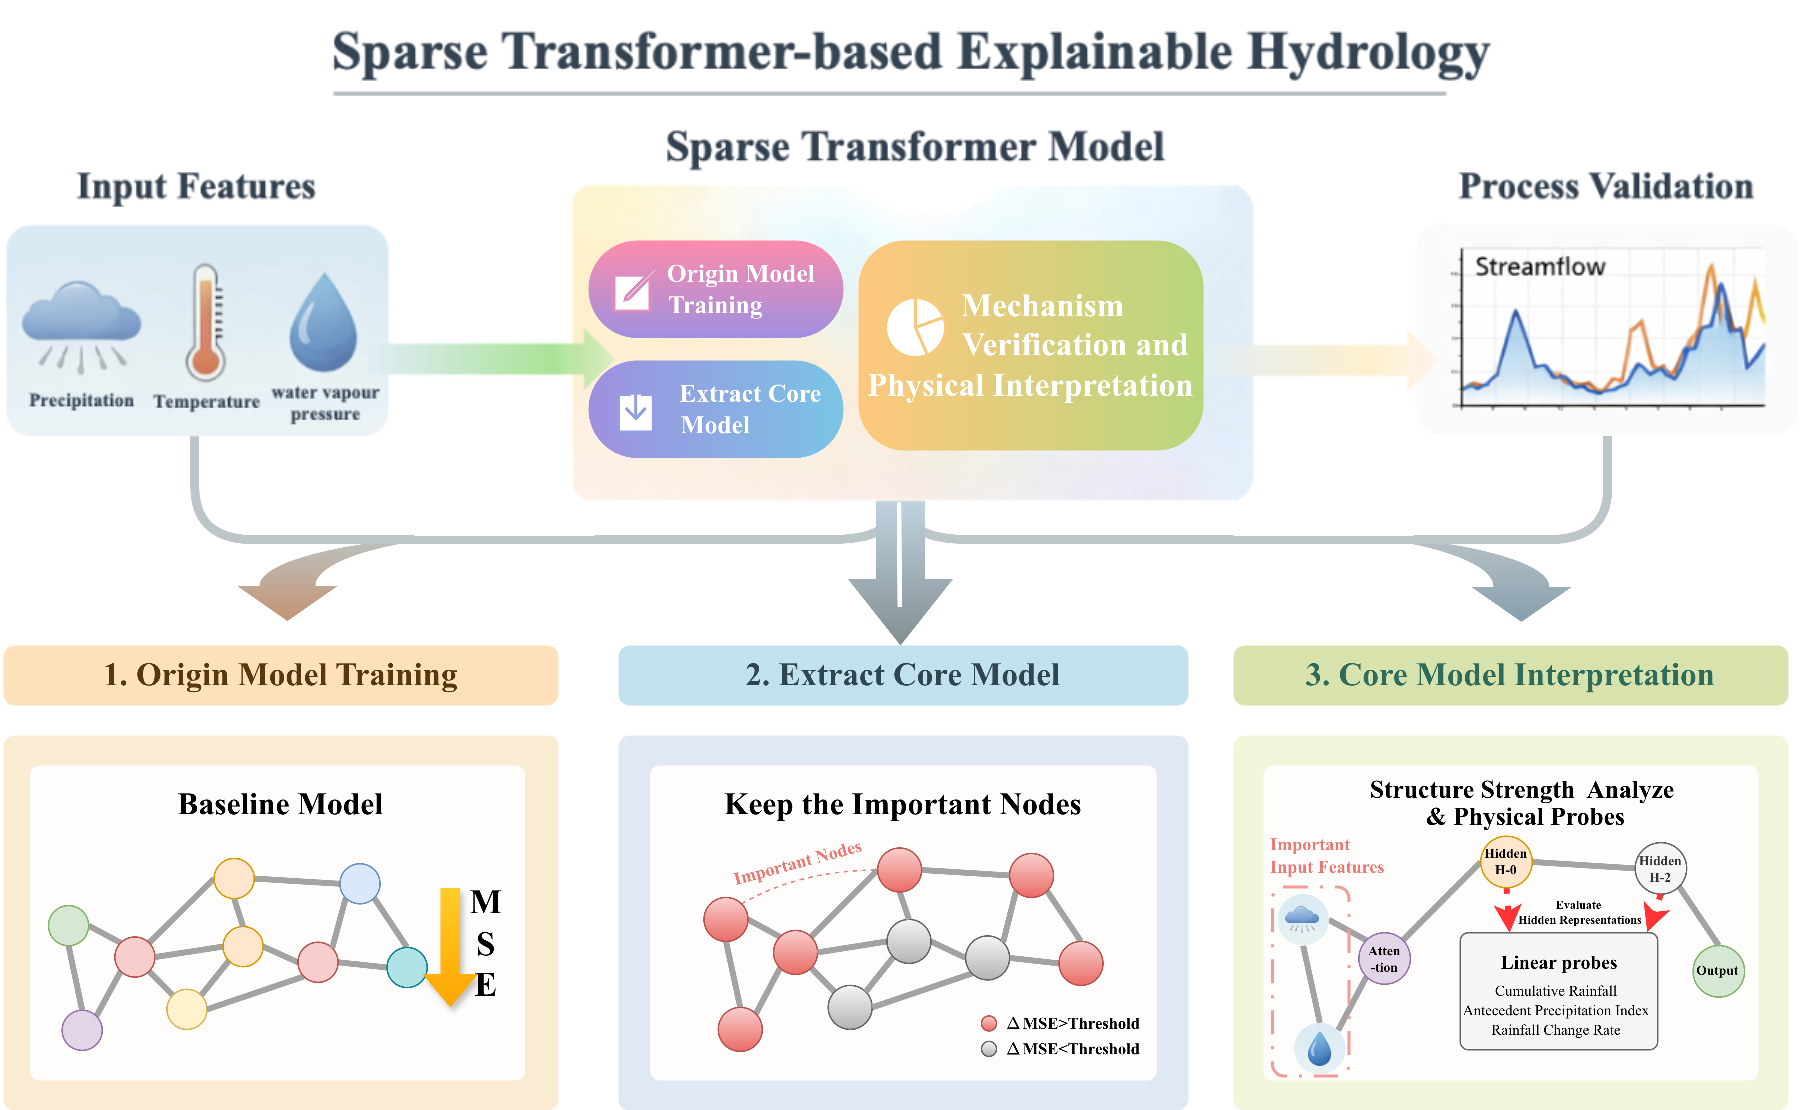
\includegraphics[width=\textwidth]{../Figures/Fig1.pdf}
    \caption{Overall architecture of the proposed STEH framework}
    \label{fig:steh}
\end{figure}

\subsection{Sparse Transformer}

The Transformer architecture has recently been introduced into hydrological time-series modeling because its self-attention mechanism can effectively capture long-range temporal dependencies in hydro-meteorological sequences\cite{LIU2024131389}. In streamflow prediction, antecedent rainfall, temperature, and soil moisture conditions jointly influence discharge responses across multiple time lags, making long-term dependency modeling particularly important\cite{li2024application}. The Transformer assigns different weights to each input feature through the self-attention mechanism, automatically learning the relationships between different time steps\cite{dumontet2026_Transformer_nc}.

\begin{figure}[ht]
    \centering
    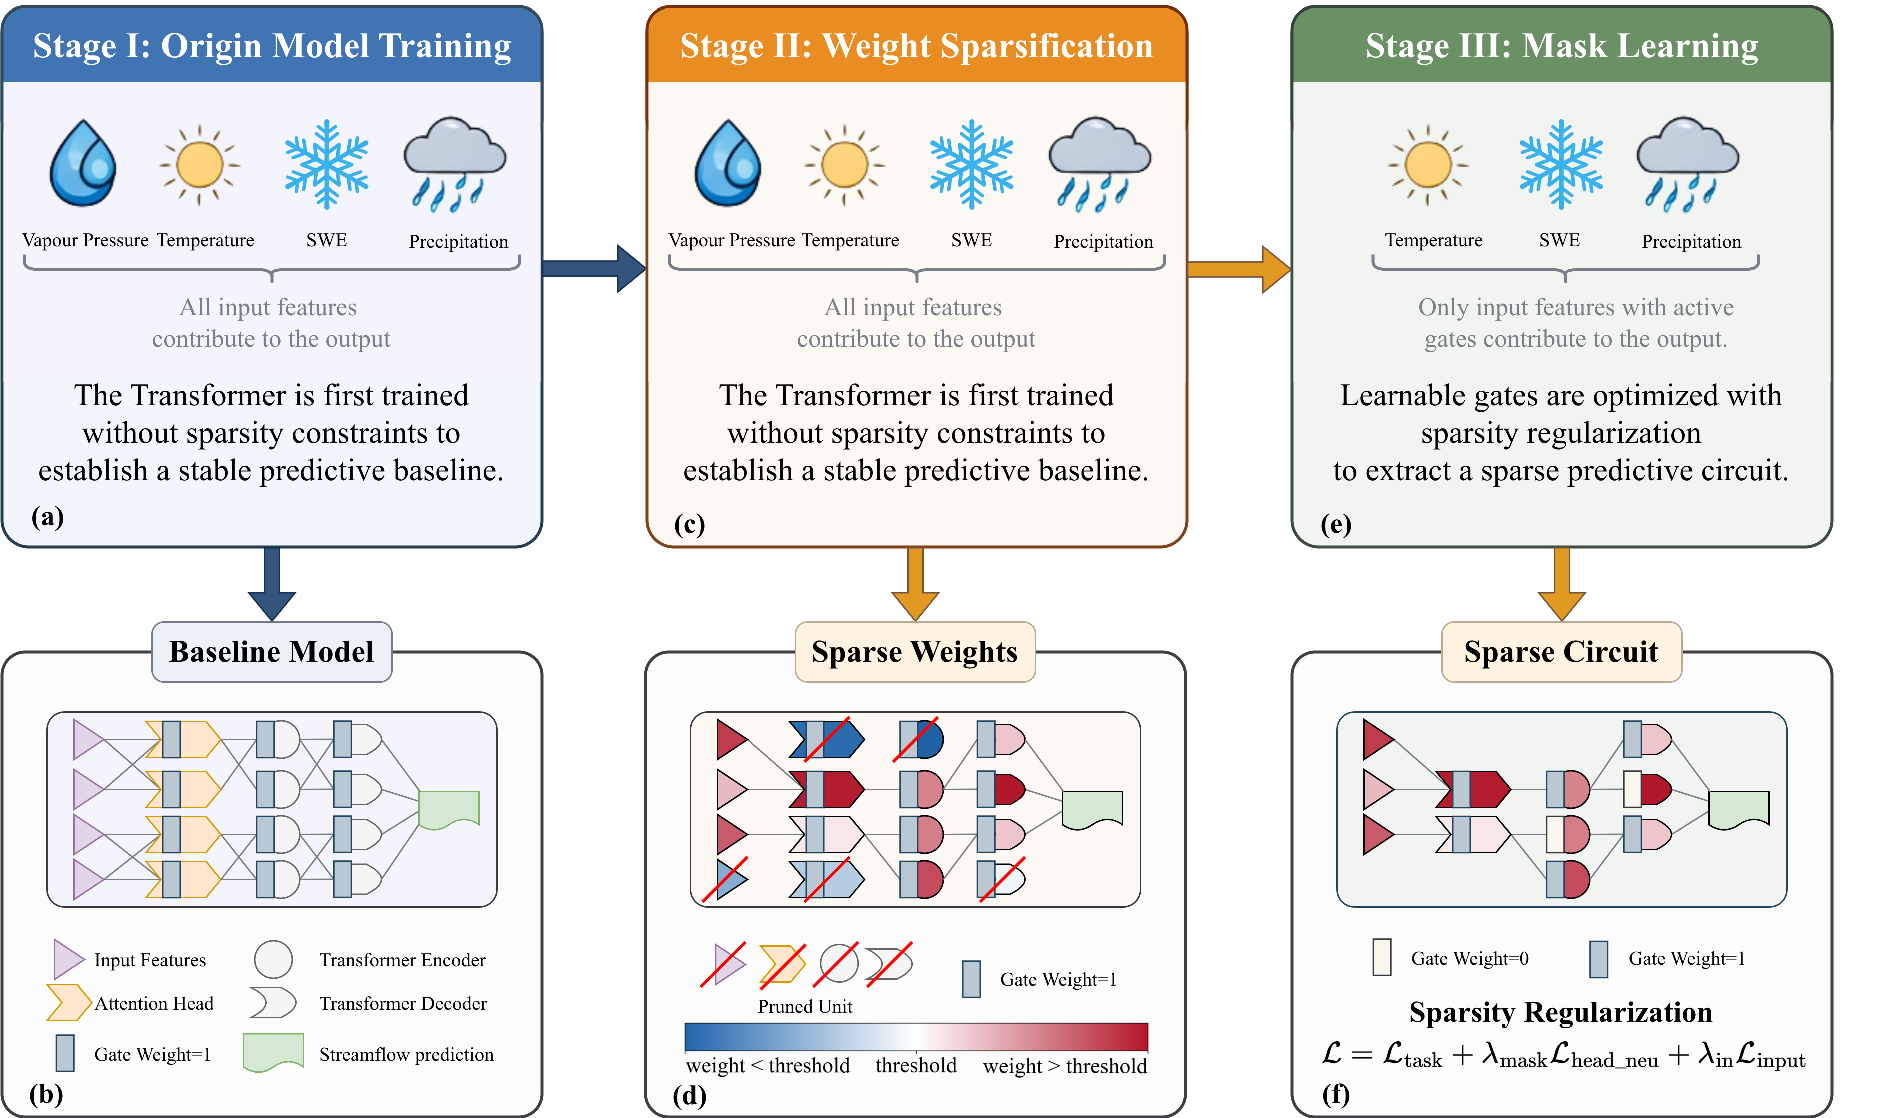
\includegraphics[width=\textwidth]{../Figures/Fig2.pdf}
    \caption{\textbf{Three-stage sparsification framework for predictive circuit discovery in Transformer.}
        The model is trained through three stages to progressively transform a dense Transformer into a sparse predictive circuit.
        (a–b) Stage I: Origin model training, where the Transformer is trained without sparsity constraints and all input features contribute to the prediction.
        (c–d) Stage II: Weight sparsification progressively prunes redundant connections according to the sparsity schedule.
        (e–f) Stage III: Mask learning optimizes learnable gates so that only a subset of input features contributes to the final prediction.
        For clarity, only a subset of connections between layers is illustrated in the figure, while the actual model remains fully connected, and decoder attention layers are omitted for simplicity.
        Note that the proposed method does not explicitly modify the network architecture; sparsity is achieved by setting weights or gates to zero, while the visual removal of units in the figure is only for illustrative purposes.
        The number of input variables shown in the figure is fewer than the actual input feature set; this simplification is adopted solely for visual clarity.
    }
    \label{fig:sparseTransformer}
\end{figure}

To enhance the interpretability of the model, we introduce a structured gating mechanism to filter input variables, attention heads, and feed-forward neurons\cite{louizos2018learningsparseneuralnetworks}. Through these gating mechanisms, we can selectively retain input features or parts of the network structure, thus enabling more efficient computation (Fig.~\ref{fig:sparseTransformer}(e--f)). By controlling the activation of gates, we are able to gradually filter out the features and pathways that have the most significant impact on the prediction. This structured sparsification approach helps the model focus on the most important inputs and computations, improving computational efficiency and enhancing model interpretability\cite{TFT}.

To avoid prematurely removing potentially important computational pathways, our training process is divided into three stages\cite{NIPS2015_three_step_pruning}:

Stage I (Origin Model Training): The model is first trained without sparsity constraints to establish a stable predictive baseline. In this stage, all input features and computational pathways are retained to ensure the model has sufficient expressive capacity (Fig.~\ref{fig:sparseTransformer}(a--b)).

Stage II (Weight Sparsification): In this stage, weight sparsification is gradually imposed, reducing redundant connections in the network. We use an annealed sparsity schedule to progressively increase the sparsity ratio, controlling which connections are pruned\cite{zhu2017prunepruneexploringefficacy}. The process sets a target sparsity ratio (from the initial $\rho_{\max}$ to the final $\rho_{\min}$) to progressively reduce the complexity of the model (\ref{fig:sparseTransformer_SI}(c--d)).

Stage III (Mask Learning): Finally, learnable gates are optimized to further refine the network (Fig.~\ref{fig:sparseTransformer_SI}(e--f)). We regularize the activation probabilities of the gates, guiding the network to select the most important input features and computational pathways\cite{NEURIPS2019_1113d7a7}. The goal is to make the computational pathways of the network more sparse by adjusting the gate activation probabilities, improving the model's inference efficiency.

These stages combined result in a compact predictive circuit that provides efficient and accurate predictions with fewer computational resources\cite{openai_weight_sparse_transformers}. Subsequently, we conduct an interpretability analysis of the model across multiple dimensions and evaluation metrics. If you are interested in the specific methods, please refer to the Supplementary Information \ref{sec:method} for further details (e.g., formal model definitions, interpretability techniques, etc.).